\documentclass{article}
\usepackage{graphicx}

\title{Labwork 6: Mapping}
\author{Nguyen Nhu Duy}
\date{}

\begin{document}

\maketitle

\section{Implementation}

Three CUDA image-processing operations were implemented using a 2D grid
and 2D blocks. For binarization, each grayscale pixel is compared with
128 and converted to either 0 or 255. Brightness control increases
the value of each RGB channel. Image blending combines two
images using
\[
Q(x,y)=c\Phi_1(x,y)+(1-c)\Phi_2(x,y).
\]
Each CUDA thread processes one pixel using its $(x,y)$ coordinates.

\section{2D Block Size Experiment}

Different 2D block sizes were tested: $(8,8)$, $(16,16)$, $(32,16)$,
$(16,32)$, and $(32,32)$. For each configuration, the execution time
was measured five times and the average value was calculated.

For binarization, the fastest average time was approximately
0.000139 s with $(32,16)$. For brightness control, the best result was
obtained with $(16,32)$ at approximately 0.000159 s.

For image blending, $(8,8)$ achieved the fastest average execution time
of approximately 0.000262 s. The other block sizes produced similar
execution times, between approximately 0.000278 s and 0.000313 s.

Overall, the best block size depends on the image-processing operation.

\begin{center}
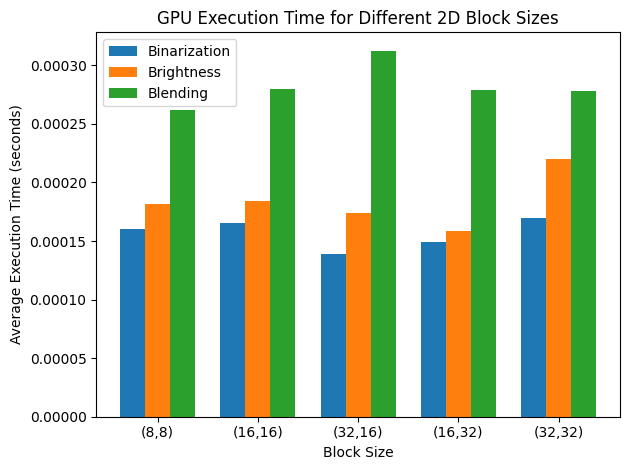
\includegraphics[width=0.85\textwidth]{block_size_comparison.png}
\end{center}

\end{document}
